\section{Second Principle: Keep the Standard Open to Correction}

An optimizer needs a way to compare alternatives. Choosing that comparison already makes decisions about value.

\subsection{A Score Contains a Settlement}

Suppose a proposal $\mathbf x$ has normalized evaluations $v_j(\mathbf x)$ on $m$ dimensions. A weighted score is
\begin{equation}
 U(\mathbf x)=\sum_{j=1}^{m}w_jv_j(\mathbf x),
 \qquad w_j\geq0,\quad\sum_jw_j=1.
\end{equation}
The score makes a tradeoff operational. It also places part of the dispute inside the weights, normalization, and functional form.

Two proposals can have the same score and quite different effects. A dimension with zero weight can change without affecting the objective. A weighted sum allows some losses to be offset by gains elsewhere. Hard constraints, priorities, or other decision rules may be more appropriate for requirements that should not be traded that way.

In a nonconvex multiobjective problem, varying positive linear weights can miss unsupported Pareto-efficient points \cite{das1997closer}. The chosen scalarization therefore affects which alternatives can emerge from the search. Keeping the original dimensions visible allows reviewers to inspect the omission.


\begin{figure}[ht]
\centering
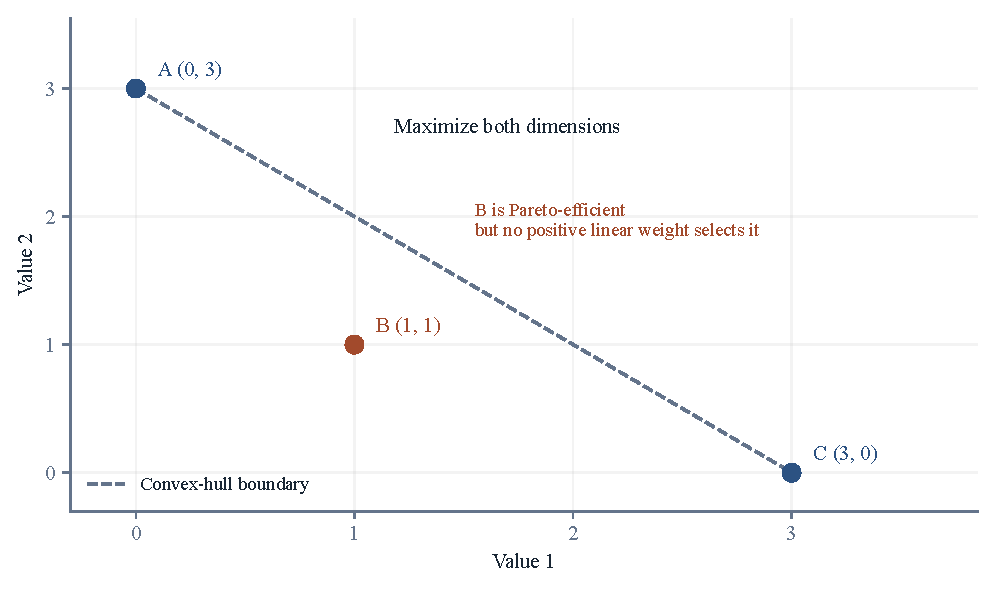
\includegraphics[width=\textwidth]{assets/unsupported-pareto.pdf}
\caption{The feasible set is $A=(0,3)$, $B=(1,1)$, and $C=(3,0)$, with both dimensions maximized. $B$ is nondominated. Yet $\max\{3w,3(1-w)\}\geq1.5>1$ for $0\leq w\leq1$, so no linear weighting selects $B$.}
\label{fig:mechanism-unsupported-pareto}
\end{figure}
Social aggregation adds another set of conditions. Arrow's theorem identifies incompatible requirements for a social ordering under an unrestricted preference domain with at least three alternatives \cite{arrow1951social}. Gibbard and Satterthwaite identify strong restrictions on deterministic strategy-proof choice under their respective assumptions \cite{gibbard1973manipulation,satterthwaite1975strategy}.

The theorems clarify tradeoffs in institutional design. They leave room for restricted domains, other information, different procedures, and explicit compromises. Their assumptions identify which institutional tradeoffs must be made explicit.

No-free-lunch results likewise concern averaging over specified spaces of objective functions \cite{wolpert1997no}. Real systems succeed by exploiting structure in particular task distributions. Representation, data, and objectives carry those commitments into deployment.

When a proxy becomes a target, optimization can exploit the gap. A game agent can collect reward without completing the intended task \cite{amodei2016concrete}. An organization can improve reported output while weakening the service the report was meant to describe.

The response is to expose the settlement: retain underlying measures, investigate gaming, permit challenge, and revise the objective when the proxy fails.

\subsection{What Formal Limits Establish}

Gödel's incompleteness theorems, Turing's undecidability result, Tarski's undefinability result, and Rice's theorem locate different boundaries \cite{godel1931,turing1936,tarski1936wahrheitsbegriff,rice1953classes}. They are strong precisely because their objects and conditions are explicit.

A sufficiently strong, consistent, effectively axiomatized arithmetic theory has undecidable sentences. Under the usual conditions it cannot establish its own formalized consistency. A universal program cannot decide the halting of every arbitrary program. A suitable arithmetic language cannot define its own complete truth predicate in the required sense. Nontrivial extensional properties of partial computable functions are undecidable in general.

Arguments about human cognition and machine authority require additional premises. Lucas and Penrose's arguments about minds and formal systems involve additional assumptions about human and machine reasoning \cite{lucas1961minds,penrose1989emperor}.

The relevant engineering practice is to state which assumptions a guarantee uses. A proof connects an implementation to a formal specification. Requirement analysis and evidence connect that specification to a desired use. Authority and rights connect the use to an acceptable decision.

The seL4 work made important parts of the first relation machine-checkable while listing what remained assumed \cite{klein2009sel4}. A smaller trusted base improves inspectability. Questions beyond the formal specification still need their own evidence and judgment.

Static analysis illustrates the choice. Let $B$ be programs with a target property and $L$ programs reported by a tool. Then
\begin{equation}
 B\subseteq L\quad\text{means no missed positives},
 \qquad
 L\subseteq B\quad\text{means no false positives}.
\end{equation}
A terminating universal tool satisfying both for a Rice-type property would be a forbidden general decision procedure. Restricting the language or property can permit exact decisions; sound approximation, runtime monitoring, and review offer other useful arrangements.

Specific progress remains possible within general limits. The 2024 busy-beaver project established the five-state value $47{,}176{,}870$ through collaborative computation and proof work \cite{bbchallenge2024}. Undecidability of the unrestricted function did not settle that particular case.

\subsection{Evidence, Authority, and Revision}

A standard can be proposed by a person or machine, tested by software, challenged by evidence, and authorized through an institution. The legitimacy of adopting it depends on the relevant rights and procedures.

The normative requirement advanced here is openness to correction. People affected by a consequential decision need a way to learn its basis, challenge a relevant error, and seek a remedy. Experts need ways to revise a standard when the world exposes a failure.

The stakes and distribution of power supply the case for this principle. Its justification belongs in the open, alongside the technical evidence.

\subsection{Where Scarcity May Move}

If routine production becomes cheaper, some complementary functions can become more important: reliable verification, well-supported care, field judgment, long-term education, and institutions able to resolve consequential disputes.

Each has a different constraint. Verification needs evidence appropriate to a claim. Care needs time, skill, access, and sometimes a particular relationship. Field judgment needs information and an effective action position. Education needs a path by which learners develop capabilities rather than merely submit outputs.

These functions offer candidates for investment. Parts of each function can improve through tools. The useful criterion is which necessary function remains difficult to supply at the required quality.

Scarcity also fails to guarantee high pay. A caregiver's bargaining power, a public budget, or a family's income can matter more than the activity's necessity. Productivity differences can raise relative service costs without automatically raising the worker's reward.

The second principle therefore has two parts. Keep the chosen standard open to evidence and challenge. Then examine whether the people maintaining its necessary functions actually receive the resources and authority the function requires.
